
\section{Implementation}
\begin{figure}[t]
    \begin{minipage}{1.0\columnwidth}
        \centering
        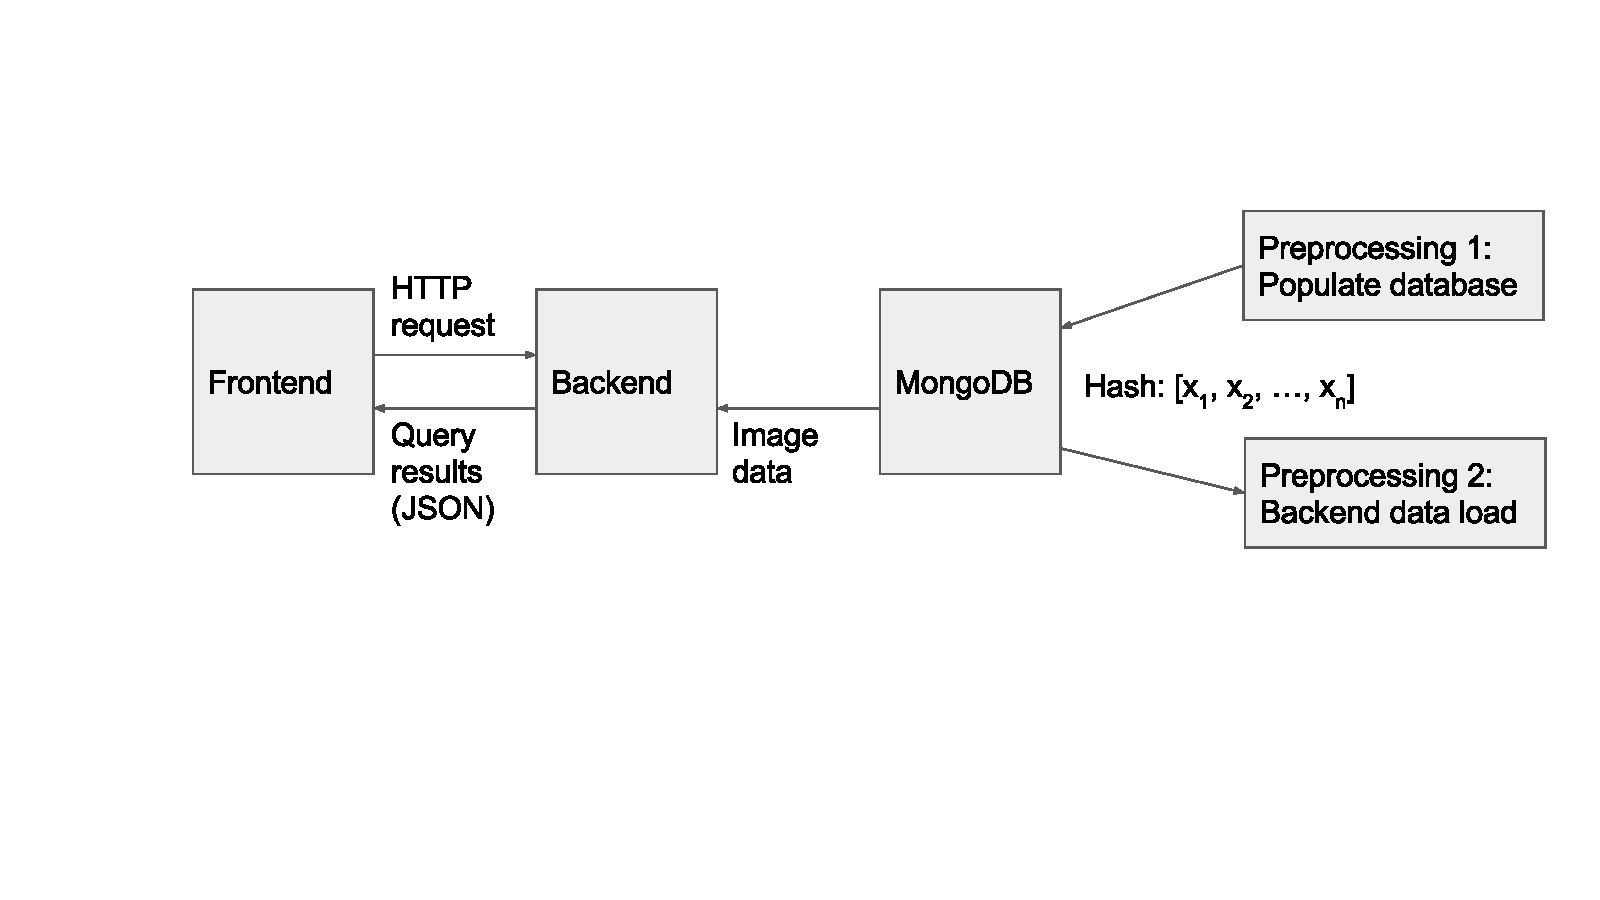
\includegraphics[width=0.9\columnwidth]{figs/system-design}
    \end{minipage}
    \caption{Overall System Design}
    \label{fig:system-design}
\end{figure}
The system works as follows:\\
    1. The frontend sends a series of query images (include and/or exclude) to the backend. \\
    2. The backend calculates the cosine distance from the hash of every query image to the hash of every image in the database. \\
    3. The backend then hands off these distances to post-processing where the algorithms mentioned in Section \ref{sec:algo}.

\subsection{Frontend Design}
The frontend is implemented using Meteor~\cite{coleman2015discover} (special thanks to Michael Kaminsky).
The frontend allows users to see their entire image collection and select images to use as positive
and negative queries by clicking on them.

\subsection{Backend Design}
The backend is implemented in Python and accepts HTTP requests from the frontend.
The backend is persistent and uses a request-based model, rather than invoked upon every new user query,
which is done for performance reasons.
The main mechanism to calculate cosine distances between image hashes is to use the cdist function in the
scipy~\cite{jones2001open} library for Python.

Further work includes optimizing this calculation, as it is currently implemented not as matrix multiplication
but as for loops.
The reason for this seems to be to minimize floating point error, but an application such as this is very
tolerant to rounding and quantization, so we believe there are further performance gains possible on this
operation.

\subsection{Optimizations}
\label{sec:optimizations}
One of the goals of the system was to enable fast (<1s) queries of the image set in order to achieve
a good user experience.
In order to reach this performance goal, we implemented 2 preprocessing steps.
The first preprocessing step uses TensorFlow~\cite{abadi2016tensorflow} to generate hashes for each image and
store them in MongoDB.
The hash in this implementation of imagematch is the output of the pool\_3 layer of the Inception
model~\cite{szegedy2015going} pretrained on the 2012 ImageNet dataset.
Due to time constraints, using other layers was not explored in depth in this project and is left for
future work.
One possible difficulty in using the output of earlier layers is that the amount of memory and computation
increases as the size of the hash increases, and the activations output by earlier layers are larger than
the output of pool\_3.

The second preprocessing step pre-loads all of the hashes from MongoDB into a matrix stored by the backend.
This allows queries to occur without any of the overhead associated with marshalling data into different formats.

\section{Evaluation}
\label{sec:eval}
The evaluation of the query result quality and the performance were done completely separately.
The former was done using user studies and on a hand-picked image set (dataset 1), while the latter was done
on an arbitrarily chosen subset of the ImageNet dataset~\cite{krizhevsky2012imagenet} (dataset 2).

Dataset 1 is of modest size (about 150 images), whereas dataset 2 varies in size from 10,000 to 300,000 images.
Due to time constraints, image sets larger than 300,000 images were left for future work.

\subsection{Testbed}
All performance experiments were run on a server with 128gb of DRAM and 2x Intel Xeon E5-2683, each of which has 32 hardware threads running at 2.1GHz.
Due to time constraints, all results shown are of a single trial.

\subsection{Performance Evaluation}
%real    378m0.593s
%user    11362m13.508s
%sys     51m41.416s
To evaluate performance, we used 300,000 arbitrarily chosen images from the ImageNet dataset.
We believe that this number is representative of a typical user's photo collection.
The first preprocessing step takes 189 hours of CPU time (about 6 hours on our testbed) to compute the hashes of 300,000 images and load them into the database.

\begin{figure}[t]
    \begin{minipage}{1.0\columnwidth}
        \centering
        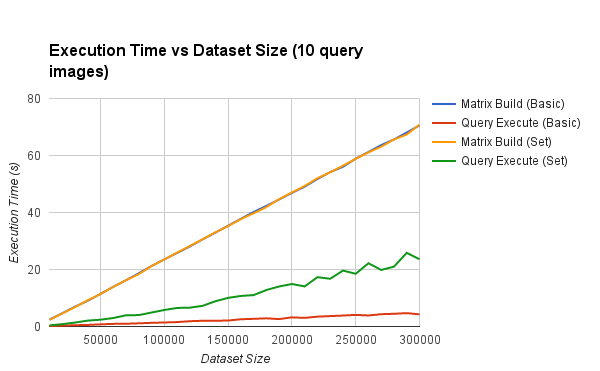
\includegraphics[width=0.9\columnwidth]{figs/vary-dataset}
    \end{minipage}
    \caption{Performance varying dataset size on a set of 10 queries.}
    \label{fig:vary-dataset}
\end{figure}
Figure~\ref{fig:vary-dataset} describes the execution time (wall clock) for both Preprocessing Step 2~\ref{sec:optimizations} and the actual query execution.
The matrix construction step (Preprocessing Step 2) grows at a linear rate as the number of dataset images increases, which is expected.

During query execution, we notice that the set search experiences much higher growth in execution time as the dataset size increases than basic search.
This is because the amount of post-processing after the distance calculation is much larger for the set search.

For 10 queries and 300,000 images, basic search achieves just over 4 seconds to execute a single query, which is on the long side (by an order of magnitude.
The reason for this is because the overhead of data type/format marshalling in python is dominating the cost of actual computation. Future work includes
implementing this in a lower level language and getting performance down to where it should be.

\begin{figure}[t]
    \begin{minipage}{1.0\columnwidth}
        \centering
        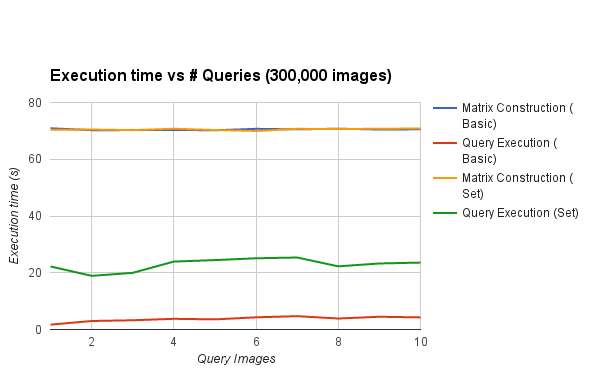
\includegraphics[width=0.9\columnwidth]{figs/vary-queries}
    \end{minipage}
    \caption{Performance varying queries on a dataset of 300,000 images.}
    \label{fig:vary-queries}
\end{figure}

Similar to Figure~\ref{fig:vary-dataset}, Figure~\ref{fig:vary-queries} shows the execution time (wall clock) for Preprocessing Step 2 and the actual query execution.

The matrix construction step (Preprocessing Step 2) is not affected by the number of queries.

The query execution time appears to grow very slowly as the number of queries increases for basic search.

However, the data turned out to be inconclusive for set search.
Again, in both cases the amount of time taken to compute the result of the query is an order of magnitude longer than it should be
(a matrix multiplication of this size should take milliseconds, not seconds).

These performance overhead issues are not addressed in this project because the scope of this project is primarily
algorithmic exploration with some smaller emphasis on performance.
Further work involves more emphasis on performance to run queries over 1,000,000 images in less than 1 second.

\subsection{Quality Evaluation}

\section{Conclusion}
